\documentclass[]{article}
\usepackage{geometry}[margin=1in]
\usepackage{amsmath}
\usepackage{amsfonts}
\usepackage{physics}
\usepackage{graphicx}
\usepackage{setspace}
\usepackage{pdfpages}
\usepackage{color, soul}



% MATLAB Formating Code
\usepackage[numbered,framed]{matlab-prettifier}
\lstset{style=Matlab-editor,columns=fullflexible}
\renewcommand{\lstlistingname}{Script}
\newcommand{\scriptname}{\lstlistingname}


% Table of contents /hyperlinks setup
\usepackage{hyperref}
\hypersetup{colorlinks=true, linkbordercolor = {white}}

\setlength\parindent{0pt}

\newcommand{\KF}{Kalman Filter}
\newcommand{\EKF}{Extended \KF}
\newcommand{\CT}{Continuous-Time}
\newcommand{\DT}{Discrete-Time}
\newcommand{\DTKF}{\DT \ \KF}
\newcommand{\LTI}{Linear Time-Invarient}
\newcommand{\SDS}{Sampled Data System}


\newcommand{\xHatPre}{\hat{x}_k^-}
\newcommand{\xHatPost}{\hat{x}_k^+}

\newcommand{\DARE}{\DT \ Algebraic Riccati Equation}
\newcommand{\CARE}{\CT \ Algebraic Riccati Equation}

\newcommand{\sectionname}{Section}
\newcommand{\subsectionname}{Subsection}
\newcommand{\subsubsectionname}{Subsubsection}
\renewcommand{\figurename}{Fig.}



\title{MECH 6325 - Final Project}
\author{Jonas Wagner}
\date{2020, December 4}


\begin{document}

\maketitle

\begin{abstract}
	In the assignment, multiple dynamic systems are considered and different Kalman filters are developed to estimate the states of the system. In problem 1, a standard \DTKF \ process is used to monitor the population and food supply of Wombats. In problem 2, a basic RLC circuit with process and measurement noise is observed with a Recursive \KF. In Problem 3, the steady-state \KF \ is explored by solving the \CARE \ for different system definitions. In Problem 4, a simple second-order \SDS \ is observed with a \DTKF. In Problem 5, a nonlinear model of an orbiting satellite is observed using both a Linear Hybrid \KF \ and a Hybrid Extended \KF.
\end{abstract}

\newpage

\setstretch{0.9}
\tableofcontents
\setstretch{1}

\newpage
\section{Problem 1 - Wombat Population}
	
	A linear system describing the population and food supply for wombats is described as follows:
	\begin{equation}
		\begin{aligned}
			p_{k+1} &= \frac{1}{2} p_k + 2 f_k\\
			f_k		&= f_0 + w_k\\
			y_k		&= p_k + v_k\\
		\end{aligned}
	\end{equation}
	where $p_k$ and $f_k$ are the Wombat Population and food supply respectively; $f_0$ is the constant mean food supply; $y$ is the measurement of wombat population; additionally, $w$ and $v$ are the process and measurement noise respectively.
	
	The process noise $w$ and measurement noise $v$ are defined as:
	\begin{equation}
		\begin{aligned}
			w &\sim (0,Q), \ Q = 10\\
			v &\sim (0,R), \ R = 10\\
		\end{aligned}
	\end{equation}
	
	The initial states of the system are defined as:
	\begin{equation}
		\begin{aligned}
			p_0 &= 650\\
			f_0 &= 250\\
		\end{aligned}
	\end{equation}
	
	A standard \DTKF \ is constructed for the system with the following initial conditions and covariance:
	\begin{equation}
		\begin{aligned}
			&\hat{p}_0 = 600, &\boldmath{E}[(\hat{p}_0 - p_0)^2] = 500\\
			&\hat{f}_0 = 200, &\boldmath{E}[(\hat{f}_0 - f_0)^2] = 200\\
		\end{aligned}
	\end{equation}
	
	\newpage
	\subsection{Modeling Method 1}\label{sec:pblm1_method1}
		The system can be written in standard form as:
		\begin{equation}
			\begin{aligned}
				x_{k+1} &= F x_k + G u + L w\\
				y_k		&= H x_k + v
			\end{aligned} \label{eq:Standard_SS_Model}
		\end{equation}
	
		where $x_k$ is defined as:
		\begin{equation}
			x_k = \mqty[p_k\\ f_k]
		\end{equation}
		
		For the first modeling method, it is taken that the food supply is described as stated in the problem, $f_{k+1} = f_0 + w$, so the system matrices are defined as:
		
		\begin{equation}
			\begin{aligned}
				&F = \mqty[\frac{1}{2} & 2\\ 0 & 0] \ \ \ G = \mqty[0\\ 1] \ \ \ L = \mqty[0\\ 1]\\
				\\
				&H = \mqty[1 &0] \ \ \ u_k \equiv f_0, \ \forall \ k
			\end{aligned}
		\end{equation}
		
		A standard \DTKF \ is then implemented as described in \subsectionname \ \ref{sec:DTKF}. The code to implement this can be found in \scriptname \ \ref{script:pblm1} within \appendixname \ \ref{apx:MATLAB_Code}. The results are seen in \figurename \ \ref{fig:pblm1resultsmethod1}.\\
		
		\begin{figure}[h]
			\centering
			\makebox[\textwidth][c]{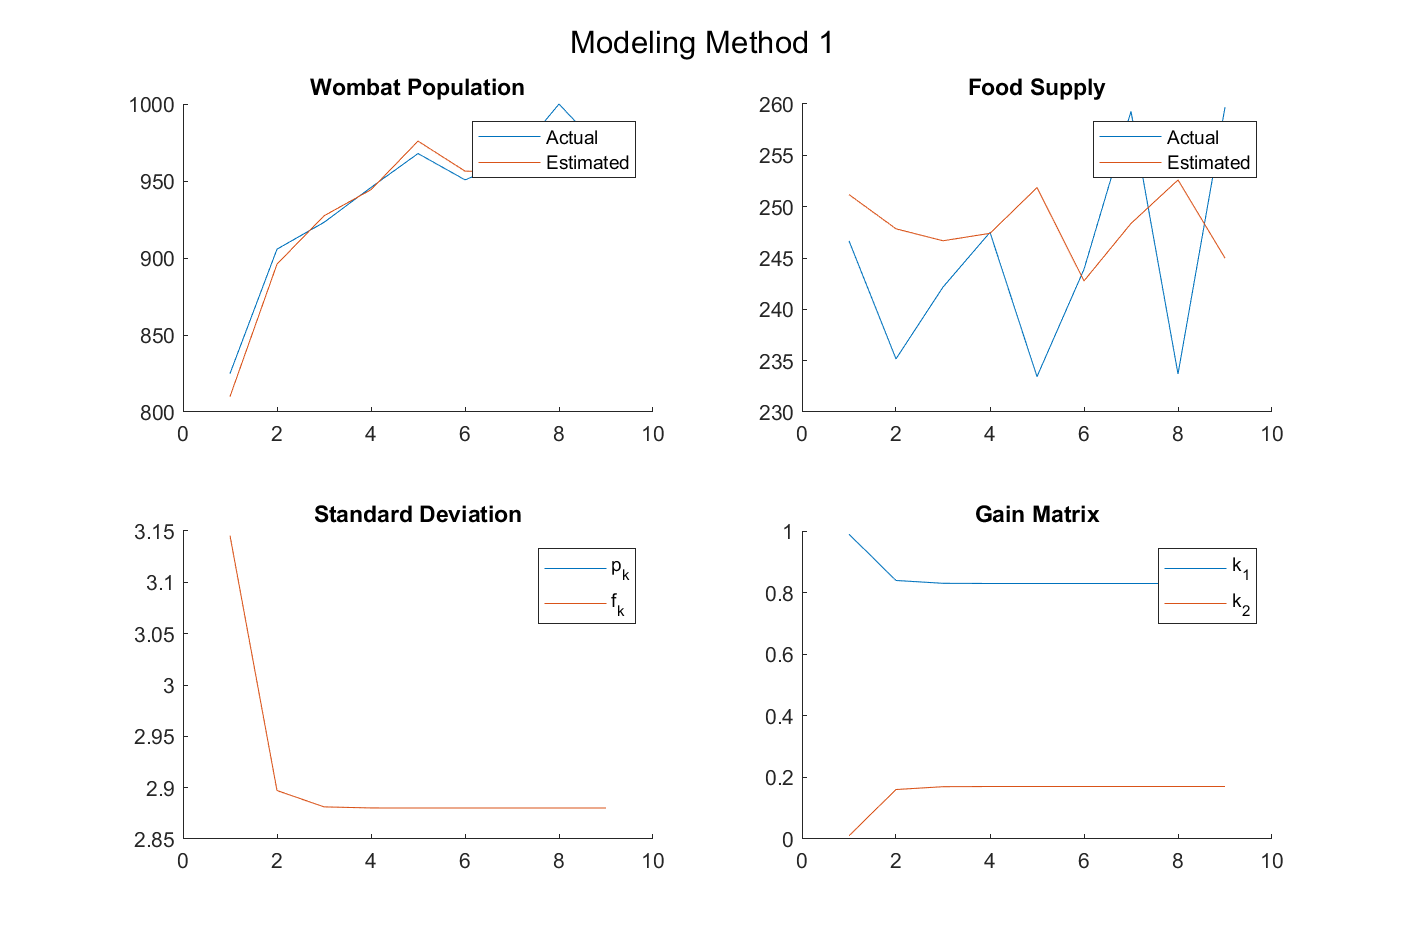
\includegraphics[height=0.45\textheight]{MATLAB/fig/pblm1_results_method1}}
			\caption{Simulation results for problem 1 using modeling method 1}
			\label{fig:pblm1resultsmethod1}
		\end{figure}
				
	\newpage
	\subsection{Modeling Method 2}\label{sec:pblm1_method2}
		The second method of modeling is also based on the same structure as \subsectionname \ \ref{sec:pblm1_method1}, but instead of a constant input, $f_{k+1} = f_0 + w$, the previous state is used, $f_{k+1} = f_k + w$. This therefore defines these new state matrices:
		\begin{equation}
			\begin{aligned}
				&F = \mqty[\frac{1}{2} & 2\\ 0 & 1] \ \ \ G = \mqty[0\\ 0] \ \ \ L = \mqty[0\\ 1]\\
				\\
				&H = \mqty[1 &0]
			\end{aligned}
		\end{equation}
	
		A standard \DTKF \ is then implemented as described in \subsectionname \ \ref{sec:DTKF}. The code to implement this can be found in \scriptname \ \ref{script:pblm1} within \appendixname \ \ref{apx:MATLAB_Code}. The results are seen in \figurename \ \ref{fig:pblm1resultsmethod2}.
		
		\begin{figure}[h]
			\centering
			\makebox[\textwidth][c]{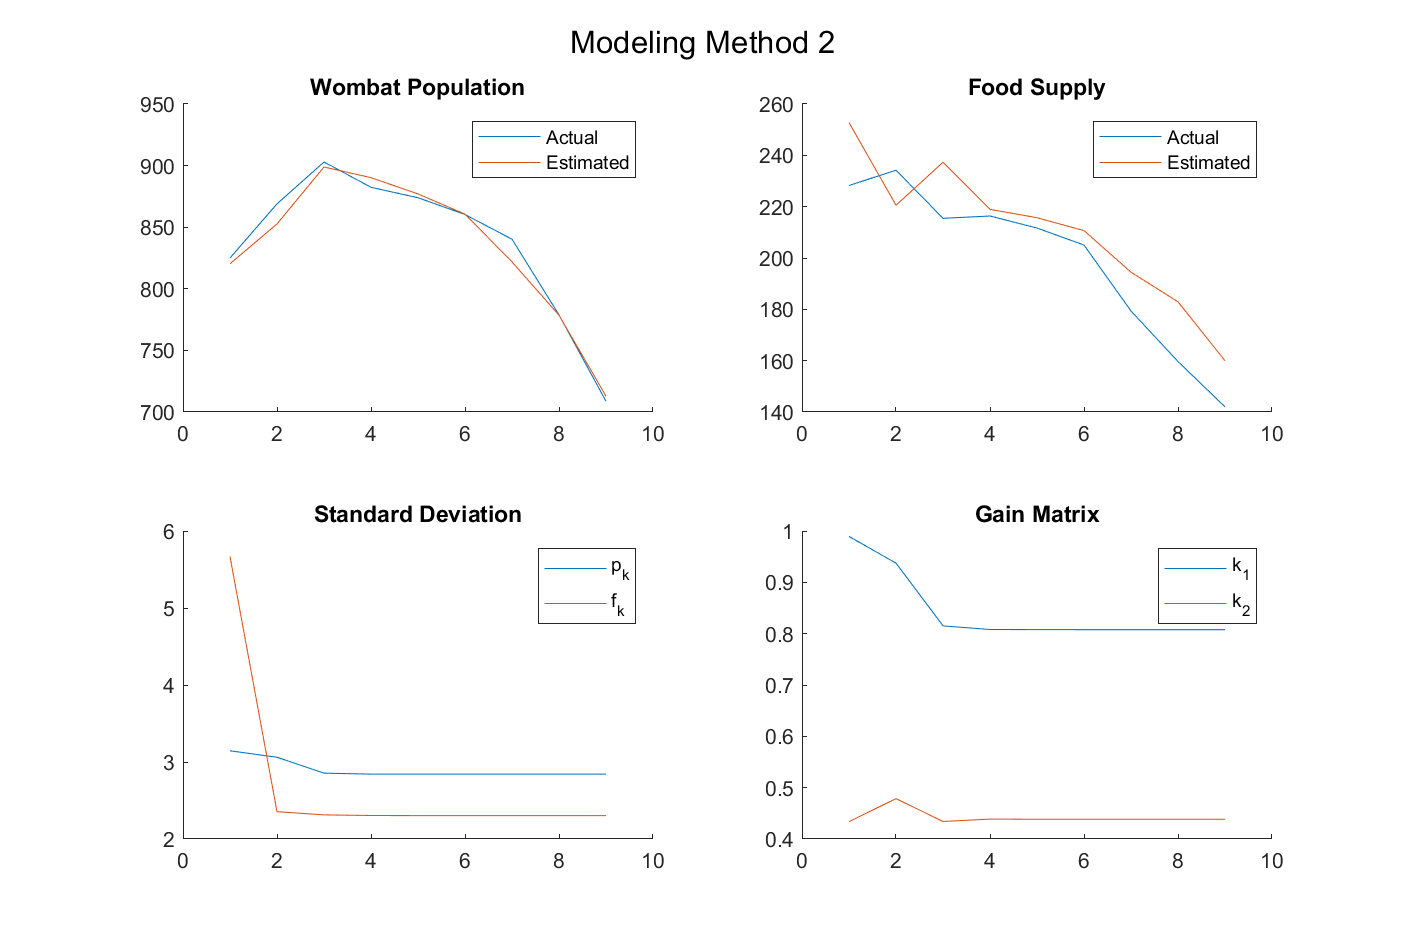
\includegraphics[height=0.5\textheight]{MATLAB/fig/pblm1_results_method2}}
			\caption{Simulation results for problem 1 using modeling method 2}
			\label{fig:pblm1resultsmethod2}
		\end{figure}
	
	
	\newpage
	\subsection{\DTKF}\label{sec:DTKF}
		The simulation of the \DTKF \ is done using a separate function that takes the parameters of the \DT \ \LTI \ system, noise properties, initial conditions, and simulation parameters. It then follows the following procedure to produce and return the actual, measured, and estimated states for each step alongside \KF \ values at each step.
		\begin{enumerate}
			\item Initialize the following:
				\begin{enumerate}
					\item Arrays that store the data for each step: X, Y, K, X\_hat\_pre, X\_hat\_post, P\_pre, P\_post\\
					\item Local variables for each iteration: x, y, p\_pre, p\_post, u, x\_hat\_pre, k, x\_hat\_post
\begin{lstlisting}
x = x_0;
y = H * x + R * randn;
p_pre = P_0;
p_post = p_pre;

u = U(1);
x_hat_pre = x_hat_0;
k = p_pre * H' * inv(R);
x_hat_post = x_hat_pre;
\end{lstlisting}
				\end{enumerate}
			\item Begin a for loop to iterate through each time step, \lstinline{for i = 1:(N-1)}.
				\begin{enumerate}
					\item Simulate the system for one step:
\begin{lstlisting}
u = U(i);
x = F * x + G * u + L * Q * randn;
y = H * x + R * randn;
\end{lstlisting}
					\item Perform the standard \DTKF \ update equations:
\begin{lstlisting}
p_pre = F * p_post * F' + L' * Q * L;
k = p_pre * H' * inv(H * p_pre * H' + R);
x_hat_pre = F * x_hat_post + G * u;
x_hat_post = x_hat_pre + k * (y - H * x_hat_pre);
p_post = (eye(n) - k * H) *p_pre * (eye(n) - k * H)' + k * R * k';
\end{lstlisting}
					\item Save the local variables into the appropriate arrays.
				\end{enumerate}
			\item Set the output variables and return the simulated system and kalman filter states and values.
		\end{enumerate}
	This is implemented in MATLAB within \scriptname \ \ref{script:KF_DT}.
	
	\newpage
	\subsection{Theoretical Error Comparison}
		The theoretical steady state a priori covariance matrix for a \DTKF, $P_\infty^-$, can be solved for using the \DARE \ (DARE):
		\begin{equation}
			\begin{aligned}
				P_\infty^-= &F P_\infty^- F^T -\\
							&F (P_\infty^- H^T + M)(H P_\infty^- + H M + M^T H^T + R)^{-1} \cross\\
							&(H P_\infty^- + M^T)F^T + Q
			\end{aligned}\label{eq:DARE}
		\end{equation}
		
		This can then be used to solve for the steady-state Kalman gain, $K_\infty$:
		\begin{equation}
			K_\infty = (P_\infty H^T + M)(H P_\infty H^T + H M + M^T H^T + R)^{-1}
		\end{equation}
		
		The theoretical steady state a postari covariance matrix for a \DTKF, $P_\infty^+$, can be calculated as:
		\begin{equation}
			P_\infty^+ = (I - K_\infty H) P_\infty^-
		\end{equation}
		
		\subsubsection{Modeling Method 1:}
			This can then be applied to find the theoretical standard deviation for each state. Within \scriptname \ \ref{script:pblm1}\ the following is found for the first method:
			\begin{equation}
				\sqrt{P_\infty^-} = \mqty[2.897 & 0\\ 0 & 3.163]
			\end{equation}
			
			Comparing this to the steady-state experimental estimation error standard deviation for both states, see \figurename \ \ref{fig:pblm1stdmethod1}, there is a noticeable discrepancy for the second state. This is believed to be because the second state is not based on the previous value, so the standard deviation follows that of the directly measured state.
			
			\begin{figure}[h]
				\centering
				\makebox[\textwidth][c]{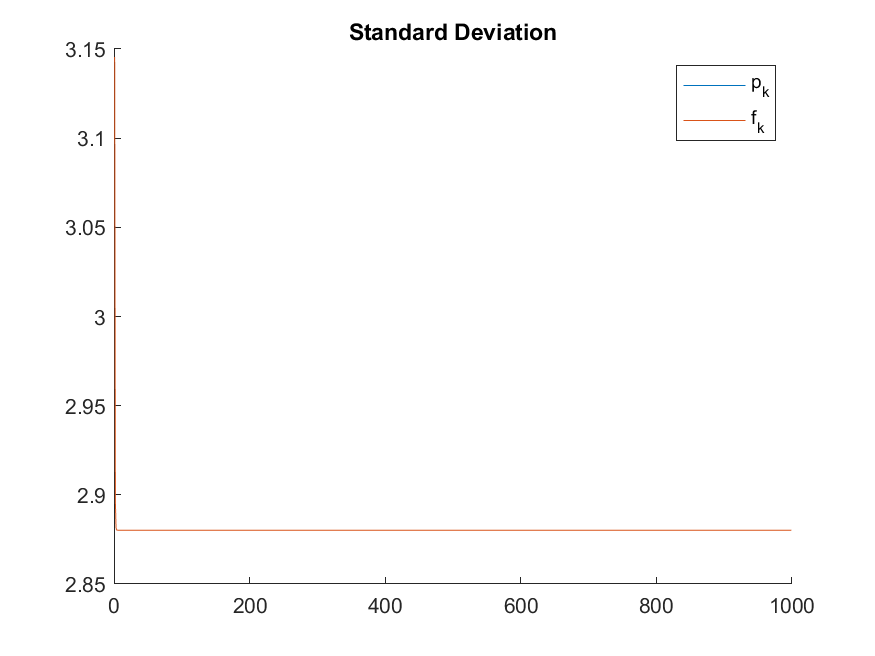
\includegraphics[height=0.35\textheight]{MATLAB/fig/pblm1_std_method1}}
				\caption{Experimental estimation error standard deviation for problem 1 using modeling method 1}
				\label{fig:pblm1stdmethod1}
			\end{figure}
			
		\subsubsection{Modeling Method 2:}
			This can then be applied to find the theoretical standard deviation for each state. Within \scriptname \ \ref{script:pblm1}\ the following is found for the second method:
			\begin{equation}
				\sqrt{P_\infty^-} = \mqty[2.9212 &1.9569\\ 1.9569 &3.4784]
			\end{equation}
			
			Comparing this to the steady-state experimental estimation error standard deviation for both states, see \figurename \ \ref{fig:pblm1stdmethod2}, there is a noticeable discrepancy for the second state. In this case, the second state has a better standard deviation then the theoretical one. This could be due to the fact that the expected value for the food-supply never deviates and is more predictable then if an input were included.
			
			\begin{figure}[h]
				\centering
				\makebox[\textwidth][c]{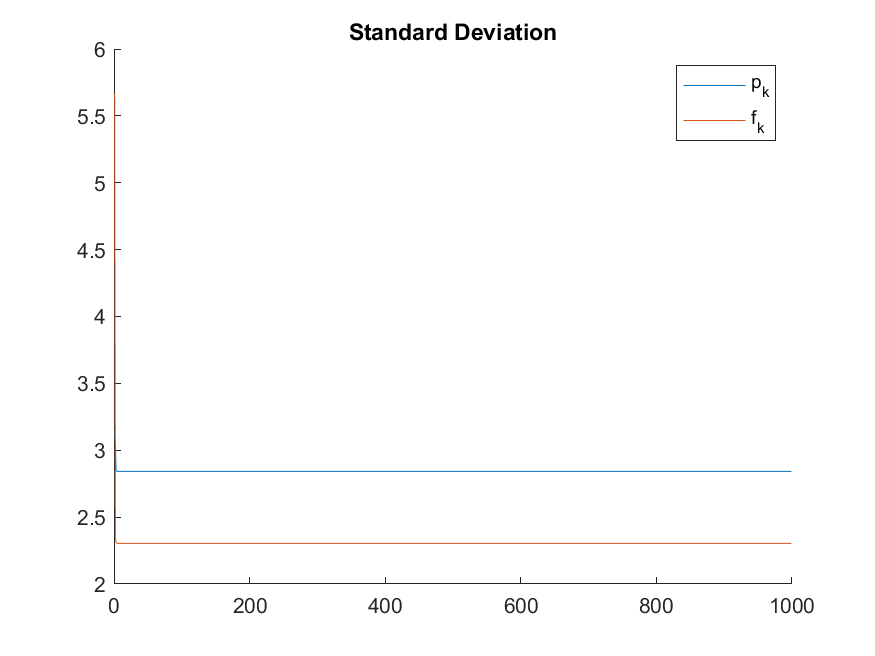
\includegraphics[height=0.35\textheight]{MATLAB/fig/pblm1_std_method2}}
				\caption{Experimental estimation error standard deviation for problem 1 using modeling method 1}
				\label{fig:pblm1stdmethod2}
			\end{figure}

\newpage
\section{Problem 2 - Electrical Network}
	Given the electrical network seen in \figurename \ \ref{fig:pblme2_circuit}, a \CT \ \LTI \ system can be developed that models the network. This can then be discretized and a sequential \KF can be developed.
	
	\begin{figure}[h]
		\centering
		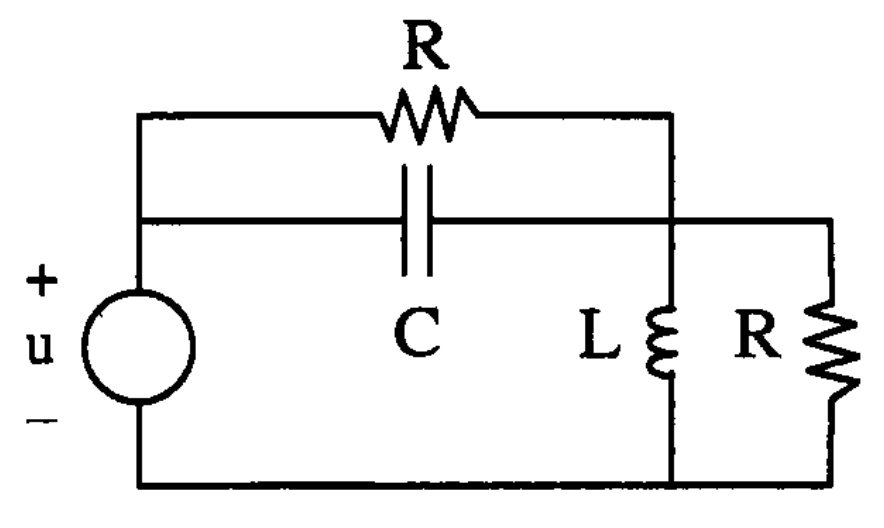
\includegraphics[width=0.5\textwidth]{fig/pblm2_fig}
		\caption{Electrical network modeling in problem 2.}
		\label{fig:pblme2_circuit}
	\end{figure}
	
	In this RLC circuit, the following parameters are defined:
	\begin{equation}
		\begin{aligned}
			R &= 100\\
			L &= 1\\
			C &= 1\\
			u &\sim (0,(3)^2)\\
		\end{aligned}
	\end{equation}
	
	It is also known that the system is relaxed at $t=0$. The system states are to be directly measured at increments of $T = 0.1$ \ s with unity variance noise and a sequential \KF \ will be used to estimate the Capacitor Voltage and Inductor Current.
	
	\subsection{System Modeling}
		Let $x$ be defined as:
		\begin{equation}
			x = \mqty[v_c\\ i_L]
		\end{equation}
		
		The system can then be modeled in the standard \CT \ \LTI \ form:
		\begin{equation}
			\dot{x} = A x + B u
		\end{equation}
		
		where $A$ and $B$ are defined as:
		\begin{equation}
			\begin{aligned}
				&A = \mqty[-2/RC & 1/C\\ -1/L & 0]&& &B = \mqty[1/RC \\ 1/L]
			\end{aligned}
		\end{equation}
		
		The input is set to the process noise term as:
		\begin{equation}
			u \equiv w \sim (0, Q_c)
		\end{equation}
		where $Q_c = 9$.
		
	\subsection{\DT \ Modeling} \label{sec:DT_sys_model}
		Equivalent \DT \ \LTI \ state-space matrices can be calculated as:
		\begin{equation}
			\begin{aligned}
				F &= e^{A T}\\
				G &= F \int_0^T I - e^{-A  \tau} \dd{\tau} B\\
				Q &= Q_c T
			\end{aligned}
		\end{equation}
		With $L = G$ and $H = I_2$, the \DT \ \LTI \ model is then defined as:
		\begin{equation}
			\begin{aligned}
				x_{k+1} &= F x_k + L w\\
				y_k		&= H x_k + v
			\end{aligned}
		\end{equation}
		where the measurement noise is defined as $v \sim (0,I_2)$.\\
		
		The system itself is calculated within \scriptname \ \ref{script:pblm2} \ and \ref{script:DiscretizeSystem}. Numerically the state matrices are defined as follows:
		\begin{equation}
			\begin{aligned}
				&F = \mqty[	0.9930 & 0.0997\\
							-0.0997& 0.9950]
				&&G = \mqty[0.0060\\ 0.0998]\\
				&H = \mqty[\imat{2}]
			\end{aligned}
		\end{equation}
	
	\subsection{Sequential \KF}
		The simulation of the Sequential \KF \ is done using a separate function that takes the parameters of the \DT \ \LTI \ system, noise properties, initial conditions, and simulation parameters. It then follows the following procedure to produce and return the actual, measured, and estimated states for each step alongside \KF \ values at each step.
		\begin{enumerate}
			\item Initialize the following:
			\begin{enumerate}
				\item Arrays that store the data for each step: X, Y, K, X\_hat\_pre, X\_hat\_post, P\_pre, P\_post, P\_all\\
				\item Local variables for each iteration: x, y, p\_pre, p\_post, u, x\_hat\_pre, k, x\_hat\_post
\begin{lstlisting}
x = x_0;
y = H * x + R * randn;
p_pre = P_0;
p_post = p_pre;

u = U(1);
x_hat_pre = x_hat_0;
k = p_pre * H' * inv(R);
x_hat_post = x_hat_pre;
\end{lstlisting}
			\end{enumerate}
			\item Begin a for loop to iterate through each time step, \lstinline{for i = 1:N}.
			\begin{enumerate}
				\item Simulate the system for one step:
\begin{lstlisting}
u = U(i);
x = F * x + G * u + L * Q * randn(size(Q,1),1);
y = H * x + R * randn(size(R,1),1);
\end{lstlisting}
				\item Perform the standard \DTKF \ time update equations:
\begin{lstlisting}
p_pre = F * p_post * F' + L' * Q * L;
x_hat_pre = F * x_hat_post + G * u;
\end{lstlisting}
				\item Initialize the measurement update loop by solving for the first a postari estimate:
\begin{lstlisting}
k(:,1) = p_pre * H(1,:)' * inv(H(1,:) * p_pre * H(1,:)' + R(1,1));
x_hat(:,1) = x_hat_pre + k(:,1)*(y(1) - H(1,:) * x_hat_pre);
p(:,:,1) = (eye(n) - k(:,1) * H(1,:))* p_pre;
\end{lstlisting}
				\item For the rest of the sensors perform measurement updates as well, \lstinline{for j in 2:r}.
\begin{lstlisting}
k(:,j) = p(:,:,j-1) * H(j,:)' * inv(H(j,:) * p(:,:,j-1) * H(j,:)' + R(j,j));
x_hat(:,j) = x_hat(:,j-1) + k(:,j-1) * (y(j) - H(j,:) * x_hat(:,j-1));
p(:,:,j) = (eye(n) - k(:,j-1) * H(j,:))* p(:,:,j-1);
\end{lstlisting}
				\item Save the local variables into the appropriate arrays.
			\end{enumerate}
			\item Set the output variables and return the simulated system and \KF states and values.
		\end{enumerate}
		This is implemented in MATLAB within \scriptname \ \ref{script:KF_Sequential}.
	
	\subsection{Simulation Results}
		The simulated results of the Sequential \KF \ for the Capacitor Voltage Estimation Variance can be seen in \figurename \ \ref{fig:pblm2estvar}.
		
		\begin{figure}[p]
			\centering
			\makebox[\textwidth][c]{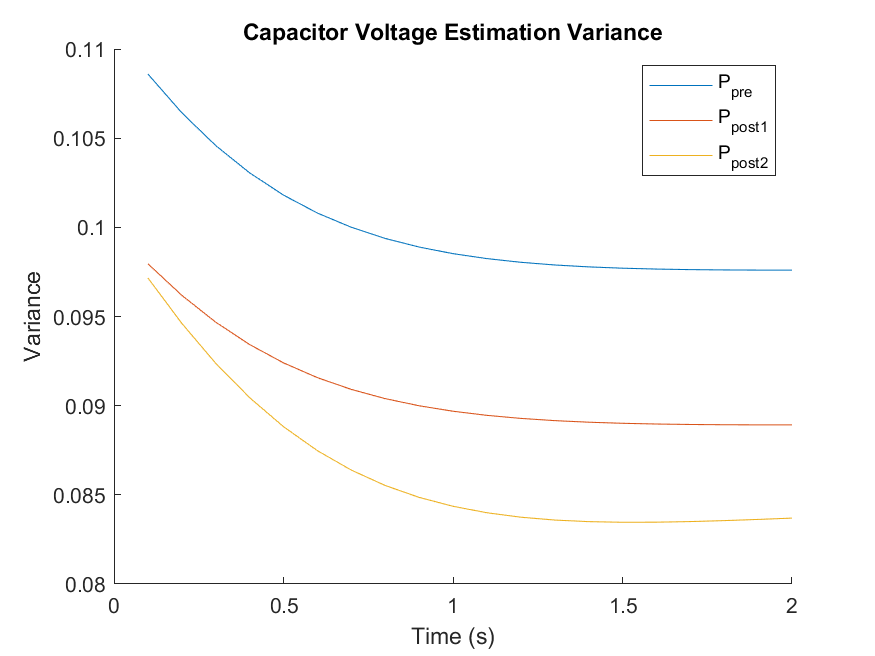
\includegraphics[width=0.7\textwidth]{MATLAB/fig/pblm2_est_var}}
			\caption{Capacitor Voltage Estimation Variance for Problem 2}
			\label{fig:pblm2estvar}
		\end{figure}
	
	\subsection{Capacitor Voltage Comparison}
		A comparison of actual, measured, and estimated Capacitor Voltages can be seen in \figurename \ \ref{fig:pblm2comparison}.
		\begin{figure}[p]
			\centering
			\makebox[\textwidth][c]{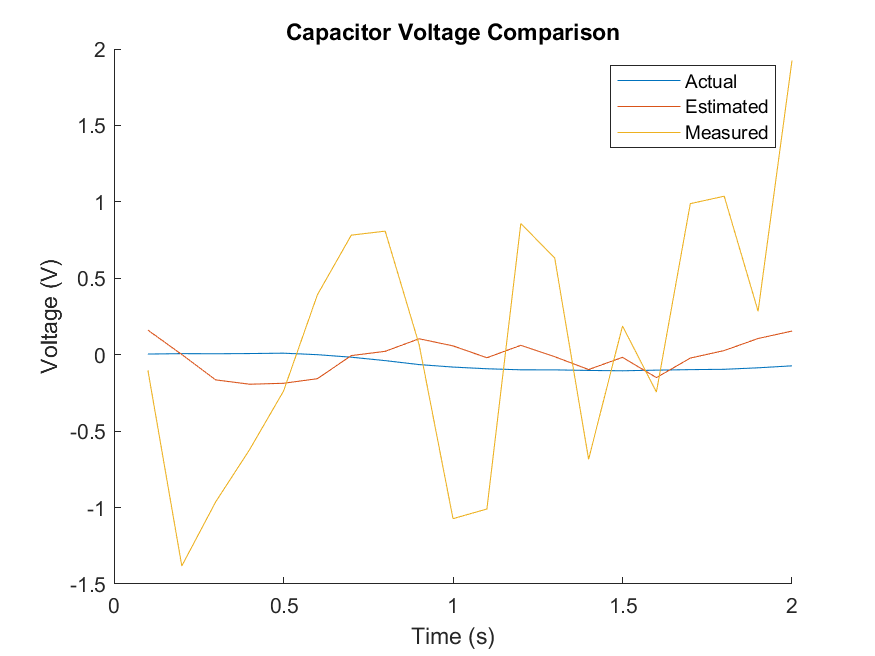
\includegraphics[width=0.7\textwidth]{MATLAB/fig/pblm2_comparison}}
			\caption{Capacitor Voltage Comparison for Problem 2}
			\label{fig:pblm2comparison}
		\end{figure}
		
		An analysis of the measurement and estimation errors yields that the standard deviations of error for each are given as follows:
		\begin{equation}
			\begin{aligned}
				\text{std}(Y_{V_C} - X_{V_C}) = 1.186\\
		 		\text{std}(\hat{X}_{V_C} - X_{V_C}) = 0.376\\
			\end{aligned}
		\end{equation}
		which clearly demonstrates the effectiveness of the \KF.


\newpage
\section{Problem 3 - Steady State Riccati Equations}
	Considering system given as:
	\begin{equation}
		\begin{aligned}
			\dot{x} &= A x + w, &&& w &\sim (0,Q)\\
			y		&= \mqty[\imat{2}] x + v&&& v &\sim (0,R),\ R = \mqty[\imat{2}]\\
		\end{aligned}
	\end{equation}
	the steady-state \KF \ can be found by solving the \CARE \ (CARE). By integrating the CARE until steady-state with various values for $A$, $Q$, and $P_0$, the existence of a stable steady-state \KF \ can be determined.
	
	\subsection{Integrating the \CARE}
	
		Integrating the \CARE \ (CARE) is done using a separate function that takes the parameters of the CARE and integration specific parameters to numerically solve for a steady-state solution to the CARE. The following procedure is followed when integrating.
		\begin{enumerate}
			\item Initialize the loop by defining:
\begin{lstlisting}
p_dot = - P_0 * C' * inv(R) * C * P_0 + A * P_0 + P_0 * A' + Q;
p = P_0 + p_dot * T;
P(:,:,1) = p;
\end{lstlisting}
			\item Begin a for loop to iterate through each time step, \lstinline{for i = 2:N}.
			\begin{enumerate}
				\item Calculate for each time step:
\begin{lstlisting}
p_dot = - p * C' * inv(R) * C * p + A * p + p * A' + Q;
p = p + p_dot * T;
\end{lstlisting}
				\item Save the current value into the output array: \lstinline{p(:,:,i)=p}
			\end{enumerate}
		\end{enumerate}
		This is implemented in MATLAB within \scriptname \ \ref{script:pblm3}.
	
	\newpage
	\subsection{Results and icare() function comparison}
		\subsubsection{Part a}
			Let,
			\begin{equation}
				A = \mqty[\dmat[0]{1,2}], \ \ Q = \mqty[\xmat{1}{2}{2}], \ \ P(0) = I_2
			\end{equation}
			
			Solving the CARE through numerical integration resulted in the following:
			\begin{equation}
				P_\infty = \mqty[2.3868 & 0.2774\\ 0.2774 & 4.2188]
			\end{equation}
			
			Solving the CARE with icare() resulted in the following:
			\begin{equation}
				P_\infty = \mqty[2.3868 & 0.2774\\ 0.2774 & 4.2188]
			\end{equation}
			
			As is evident, there is no discrepancy.
			
		\subsubsection{Part b}
			Let,
			\begin{equation}
				A = \mqty[\dmat[0]{-1,-1}], \ \ Q = \mqty[\dmat[2]{1,4}], \ \ P(0) = I_2
			\end{equation}
			
			Solving the CARE through numerical integration resulted in the following:
			\begin{equation}
				P_\infty = \mqty[0.2899 &0.5798\\ 0.5798 &1.1596]
			\end{equation}
			
			Solving the CARE with icare() resulted in the following:
			\begin{equation}
				P_\infty = \mqty[0.2899 &0.5798\\ 0.5798 &1.1596]
			\end{equation}
			
			As is evident, there is no discrepancy.
			
		\subsubsection{Part c}
			Let,
			\begin{equation}
				A = \mqty[\dmat[0]{1,1}], \ \ Q = \mqty[\dmat[2]{1,4}], \ \ P(0) = I_2
			\end{equation}
			
			Solving the CARE through numerical integration resulted in the following:
			\begin{equation}
				P_\infty = \mqty[2.2899 &0.5798\\ 0.5798 &3.1596]
			\end{equation}
			
			Solving the CARE with icare() resulted in the following:
			\begin{equation}
				P_\infty = \mqty[2.2899 &0.5798\\ 0.5798 &3.1596]
			\end{equation}
			
			As is evident, there is no discrepancy.
			
		\subsubsection{Part d}
			Let,
			\begin{equation}
				A = \mqty[\dmat[0]{1,1}], \ \ Q = \mqty[\dmat[2]{1,4}], \ \ P(0) = 0
			\end{equation}
			
			Solving the CARE through numerical integration resulted in the following:
			\begin{equation}
				P_\infty = \mqty[0.6899 &1.3798\\ 1.3798 &2.7596]
				\label{eq:pblm3d_p_infty}
			\end{equation}
			
			Solving the CARE with icare() resulted in the following:
			\begin{equation}
				P_\infty = \mqty[2.2899 &0.5798\\ 0.5798 &3.1596]
			\end{equation}
			
			As is evident, there is a discrepancy
	
	\subsection{Testing Viability of Steady-State \KF}
		Given the $P_\infty$ defined in \eqref{eq:pblm3d_p_infty}, a steady state Kalman gain can be calculated as:
		\begin{equation}
			K_\infty = P_\infty C^T R^{-1} = \mqty[0.6899 &1.3798\\ 1.3798 &2.7596]
		\end{equation}
		
		The stability of the steady-state \KF \ can then be tested by testing if $(A-K_\infty C)$ is stable.
		\begin{equation}
			(A - K_\infty C) = \mqty[0.3101 &-1.3798\\ -1.3798 &-1.7596]
		\end{equation}
		
		This can be found to be unstable as $\lambda(A - K_\infty C) = \{-2.5,1\}$, and the root at 1 is unstable.
	
\newpage
\section{Problem 4 - Second Order Sampled Data System}
	A second-order \CT \ \LTI \ system is given in standard form:
	\begin{equation}
		\begin{aligned}
			\dot{x} &= A x + L w\\
			\\
			A &= \mqty[0 & 1\\ -\omega^2 &-2\zeta\omega], \ \ L = \mqty[0\\1], \ w \sim (0,Q_c)
		\end{aligned}
	\end{equation}
	numerically, the system is defined with $\omega = 6$ rad/s, $\zeta = 0.16$, and $Q_c = 0.01$.\\
	
	The system is sampled with $T = 0.5$ s with a measurement noise $v \sim (0,R), \ R = 10^{-4}$.\\
	Additionally, the initial system and \KF \ states are known to be:
	\begin{equation}
		x(0) = \mqty[1\\1], \ \ \hat{x}(0) = x(0), \ \ P(0) = \mqty[\dmat[0]{10^{-5},10^{-2}}]
	\end{equation}
	
	\subsection{\DT \ System}
		The system is descritized as described in \subsectionname \ \ref{sec:DT_sys_model}. This results in the following numerical results:
		\begin{equation}
			\begin{aligned}
				&F = \mqty[-0.5908 &0.01873\\ -0.6743 &-0.6267] \ \ \ L = \mqty[0.04419\\ 0.0187]\\
				\\
				&H = \mqty[1 &0], \ \ Q = 0.005
			\end{aligned}
		\end{equation}
	
	\subsection{Sampled Data System \DTKF}
		The simulation of the \SDS \ \KF \ is done using a separate function that takes the parameters of the ss model, the \DT \ \LTI \ system, noise properties, initial conditions, and simulation parameters. It then follows the following procedure to produce and return the actual, measured, and estimated states for each step alongside \KF \ values and the associate time. 
		\begin{enumerate}
			\item Generate the time values for the \CT \ calcualtions: \lstinline{Xt = (T/dtdiff)*(0:(N*dtdiff));}
			\item Generate the random input signal for all time steps: \lstinline{W = randn(N*dtdiff+1,1);}
			\item Calculate the \CT \ \LTI \ system response and store to X: \lstinline{X = lsim(sys,U + Q*W,Xt,x_0)';}
			\item Initialize the following:
			\begin{enumerate}
				\item Arrays that store the data for each step: Y, K, X\_hat\_pre, X\_hat\_post, P\_pre, P\_post\\
				\item Local variables for each iteration: x, y, p\_pre, p\_post, u, x\_hat\_pre, k, x\_hat\_post
\begin{lstlisting}
x = x_0;
y = H * x + R * randn;
p_pre = P_0;
p_post = p_pre;

x_hat_pre = x_hat_0;
k = p_pre * H' * inv(R);
x_hat_post = x_hat_pre;
\end{lstlisting}
			\end{enumerate}
			\item Begin a for loop to iterate through each time step, \lstinline{for i = 1:(N-1)}.
			\begin{enumerate}
				\item Simulate the system for one step:
\begin{lstlisting}
t = i*T;
x = X(:,dtdiff*i+1);
y = H * x + R * randn;
\end{lstlisting}
				\item Perform the standard \DTKF \ equations:
\begin{lstlisting}
p_pre = F * p_post * F' + L' * Q * L;
k = p_pre * H' * inv(H * p_pre * H' + R);
x_hat_pre = F * x_hat_post + G * u;
x_hat_post = x_hat_pre + k * (y - H * x_hat_pre);
p_post = (eye(n) - k * H) *p_pre * (eye(n) - k * H)' + k * R * k';
\end{lstlisting}
				\item Save the local variables into the appropriate arrays.
			\end{enumerate}
			\item Set the output variables and return the simulated system and \KF states and values.
		\end{enumerate}
		This is implemented in MATLAB within \scriptname \ \ref{script:KF_DT_SDS}.
		
		
	\subsection{Simulation Results}
		The simulation results for the \SDS \ \KF \ can be seen in \figurename \ \ref{fig:pblm3results}. Given the simplistic nature of the system and minimal noise, the \KF \ does a good job at estimating the state; however, the sampling rate is far too slow to effectively capture the higher frequencies of the actual system response.
		
		\begin{figure}[p]
			\centering
			\makebox[\textwidth][c]{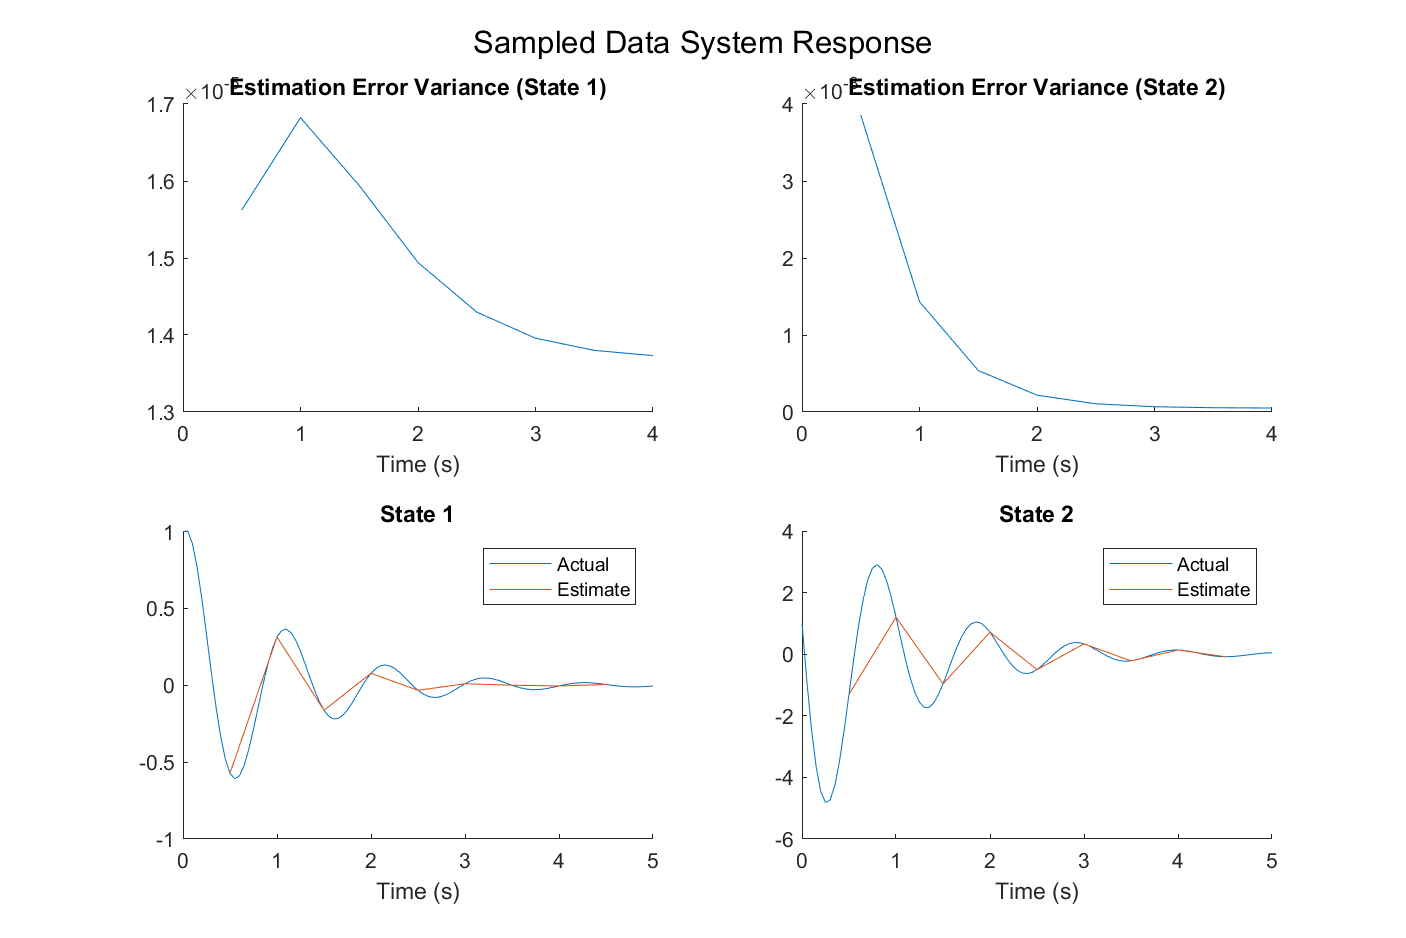
\includegraphics[width=1.2\textwidth]{MATLAB/fig/pblm4_results}}
			\caption{Simulation Results for problem 4}
			\label{fig:pblm3results}
		\end{figure}
		
		

\newpage
\section{Problem 5 - Satellite Orbit}
	All calculations and simulations were done in MATLAB, and can be seen in \scriptname \ \ref{script:pblm5}.\\
	
	A planar model for an orbiting satalite is given as:
	\begin{equation}
		\begin{aligned}
			\ddot{r} &= r \dot{\theta}^2 - \frac{G M}{r^2} + w\\
			\ddot{\theta} &= \frac{-2\dot{\theta}\dot{r}}{r}
		\end{aligned}
	\end{equation}
	where the gravitational constant $G = 6.674e-11 \qty[\frac{m^2}{kg/s^2}]$ and the mass of the earth $M = 5.98e24 [kg]$, and $w \sim (0,Q), \ Q = 10^{-6}$.
	
	\subsection{Nonlinear State-Space Model}
		Let,
		\begin{equation}
			x = \mqty[r\\ \dot{r}\\ \theta\\ \dot{\theta}]
		\end{equation}
		
		The state space model can then be defined as:
		\setstretch{1.5}
		\begin{equation}
			\dot{x} = f(x) = \mqty[\dot{r}\\
									r \dot{\theta}^2 - \cfrac{G M}{r^2} + w\\
									\dot{\theta}\\
									\cfrac{-2\dot{\theta}\dot{r}}{r}]
		\end{equation}
		\setstretch{1}
		
		\subsubsection{pblm5\_nonlin Function}
			When working with the nonlinear model, a function was defined to evaluate the system as defined in the original nonlinear state-space model. This is viewable in \scriptname \ \ref{script:pblm5_nonlin}, but the main functionality is given by:
\begin{lstlisting}
x_dot(1) = x(2);
x_dot(2) = x(1) * x(4)^2 - (G*M)/(x(1)^2) + w;
x_dot(3) = x(4);
x_dot(4) = -2*x(4)*x(2)/x(1);
\end{lstlisting}
			
	\subsection{Steady-State Radial Velocity}
		When $w = 0$, $\dot{\theta}$ can be solved for such that $r$ remains constant:
		\setstretch{1.5}
		\begin{align}
			0 = \ddot{r} &= r \dot{\theta}^2 - \cfrac{G M}{r^2}\\
			\cfrac{G M}{r^2} &= r \dot{\theta}^2\\
			\dot{\theta}_0 = \pm \sqrt{\cfrac{G M}{r^3}}
		\end{align}
		\setstretch{1}
	
	\subsection{\CT \ \LTI \ Model}
		A \CT \ \LTI \ model can be developed around an equilibrium point as follows:\\
		
		Let,
		\begin{equation}
			x_0 = \mqty[r_0\\ 0 \\ \omega_0 T \\ \omega_0]
		\end{equation}
		
		The state matrix $A$ can then be found by evaluating the Jacobian of $f(x)$ at $x_0$:
		\begin{align}
			A = \eval{\dv{f}{x}}_{x_0}
				&= \eval{\mqty[0 & 1 & 0 &0\\
						\dot{\theta}^2 + \cfrac{G M}{r^3}	&0 &0 & 2 r \dot{\theta}\\
						0	&0	&0	&1\\
						2\dot{\theta}\dot{r}	&\cfrac{-2\dot{\theta}}{r} &0 &	\cfrac{-2\dot{r}}{r}			
								]}_{x_0} \nonumber \\
			A	&= \mqty[0 & 1 & 0 &0\\
						\omega_0^2 + \cfrac{G M}{r_0^3}	&0 &0 & 2 r_0 \omega_0\\
						0	&0	&0	&1\\
						0	&\cfrac{-2\omega_0}{r_0} &0 &	0]
		\end{align}
		
		Numerically, with $r_0 = 6.57 \cross 10^6 [m]$ the $A$ matrix is calculated to be:
		\begin{equation}
			A = \mqty[0                    & 1                     & 0 & 0                \\
						4.22\cross 10^{-6} & 0                     & 0 & 1.56\cross 10^4 \\
						0                    & 0                     & 0 & 1                \\
						0                    & -3.61 \cross 10^{-10} & 0 & 0      ]
		\end{equation}
		
		The eigen-values of the $A$ matrix can be calculated to be:
		\begin{equation}
			\lambda(A) = \{0,0,\pm j 1.2 \cross 10^{-3}\}
		\end{equation}
		
		The time constant of the system $\tau$ can then be calculated as follows:
		\begin{align}
			2 \pi f_0 = \frac{2 \pi}{\tau} &= 1.2 \cross 10^{-3} \nonumber\\
			\tau &\approx 5.2 \cross 10^3 [s]
		\end{align}
		
		The largest integration step to capture the important frequencies can be estimated as:
		\begin{equation}
			0.1 \tau = 520 [s]
		\end{equation}
		
	\newpage
	\subsection{Linear Hybrid \KF} \label{sec:LinearHybridKF}
		The simulation of the Linear Hybrid \KF \ is done using a separate function that takes the nonlinear system function, the parameters of the \CT \ \LTI \ system, noise properties, initial conditions, and simulation parameters. It then follows the following procedure to produce and return the actual, measured, and estimated states for each step alongside \KF \ values and time-step values.
		\begin{enumerate}
			\item Initialize the following:
			\begin{enumerate}
				\item Arrays that store the data for each step: X, Y, K, X\_hat\_pre, X\_hat\_post, P\_pre, P\_post, Xt, sensor\_t\\
				\item Local variables for each iteration: x, p, x\_hat, k, (y)
\begin{lstlisting}
x = x_0;
p = P_0;
x_hat = x_hat_0;
k = p * H' * inv(R);
\end{lstlisting}
			\end{enumerate}
			\item Begin a for loop to iterate through each time step, \lstinline{for i = 1:N}.
			\begin{enumerate}
				\item Simulate the system for one step:
\begin{lstlisting}
t = i * sensorT;
x_dot = nonlinsys(x);
x = x + x_dot * sensorT;
y = H * x + R * randn(size(R,2),1);
\end{lstlisting}
				\item Store values into their respective arrays: X, Y, sensor\_t
				\item Perform the standard \CT \ \KF \ time update equations:
\begin{lstlisting}
x_hat_dot = A * x_hat;
x_hat = x_hat + x_hat_dot * sensorT;
p_dot = A * p + p * A' + L*Q_c*L';
p = p + p_dot * sensorT;
\end{lstlisting}
				\item Store values into their respective arrays: X\_hat\_pre, P\_pre
				\item Perform the standard \DTKF \ measurment update equations:
\begin{lstlisting}
k = p*H'*inv(H*p*H' + R);
x_hat = x_hat + k * (y - H * x_hat);
p = (eye(n)-k*H)*p*(eye(n)-k*H)' + k*R*k';
\end{lstlisting}
				\item Store values into their respective arrays: K, X\_hat\_post, P\_post
			\end{enumerate}
			\item Set the output variables and return the simulated system and \KF states and values.
		\end{enumerate}
		This is implemented in MATLAB within \scriptname \ \ref{script:KF_Hybrid_nonlinsys}.
	
	\newpage
	\subsection{Hybrid Extended \KF} \label{sec:HybridEKF}
		\hl{The Hybrid Extended Kalman Filter is nearly identical to the Linear Hybrid Kalman Filter \ version, except for the non-linear time update step}, \textbf{Step \ \ref{step:nonlin_time_update}}.\\
		
		The simulation of the Extended Hybrid \KF \ is done using a separate function that takes the nonlinear system function, the parameters of the \CT \ \LTI \ system, noise properties, initial conditions, and simulation parameters. It then follows the following procedure to produce and return the actual, measured, and estimated states for each step alongside \KF \ values and time-step values.
		\begin{enumerate}
			\item Initialize the following:
			\begin{enumerate}
				\item Arrays that store the data for each step: X, Y, K, X\_hat\_pre, X\_hat\_post, P\_pre, P\_post, Xt, sensor\_t\\
				\item Local variables for each iteration: x, p, x\_hat, k, (y)
\begin{lstlisting}
x = x_0;
p = P_0;
x_hat = x_hat_0;
k = p * H' * inv(R);
\end{lstlisting}
			\end{enumerate}
			\item Begin a for loop to iterate through each time step, \lstinline{for i = 1:N}.
			\begin{enumerate}
				\item Simulate the system for one step:
\begin{lstlisting}
t = i * sensorT;
x_dot = nonlinsys(x);
x = x + x_dot * sensorT;
y = H * x + R * randn(size(R,2),1);
\end{lstlisting}
				\item Store values into their respective arrays: X, Y, sensor\_t
				\item Perform the following nonlinear time update equations:\label{step:nonlin_time_update}
\begin{lstlisting}
x_hat_dot = nonlinsys(x_hat,0);
x_hat = x_hat + x_hat_dot * sensorT;
p_dot = A * p + p * A' + L*Q_c*L';
p = p + p_dot * sensorT;
\end{lstlisting}
				\item Store values into their respective arrays: X\_hat\_pre, P\_pre
				\item Perform the standard \DTKF \ measurment update equations:
\begin{lstlisting}
k = p*H'*inv(H*p*H' + R);
x_hat = x_hat + k * (y - H * x_hat);
p = (eye(n)-k*H)*p*(eye(n)-k*H)' + k*R*k';
\end{lstlisting}
				\item Store values into their respective arrays: K, X\_hat\_post, P\_post
			\end{enumerate}
			\item Set the output variables and return the simulated system and \KF states and values.
		\end{enumerate}
		This is implemented in MATLAB within \scriptname \ \ref{script:KF_Extended_Hybrid}.
	
	
	\subsection{Simulation Results}
		\subsubsection{Linear Hybrid \KF}
		The Linear Hybrid \KF \ was simulated using \subsectionname \ \ref{sec:LinearHybridKF}. The system response can be seen in \figurename \ \ref{fig:pblm5resultslin}.
		\begin{figure}[h]
			\centering
			\makebox[\textwidth][c]{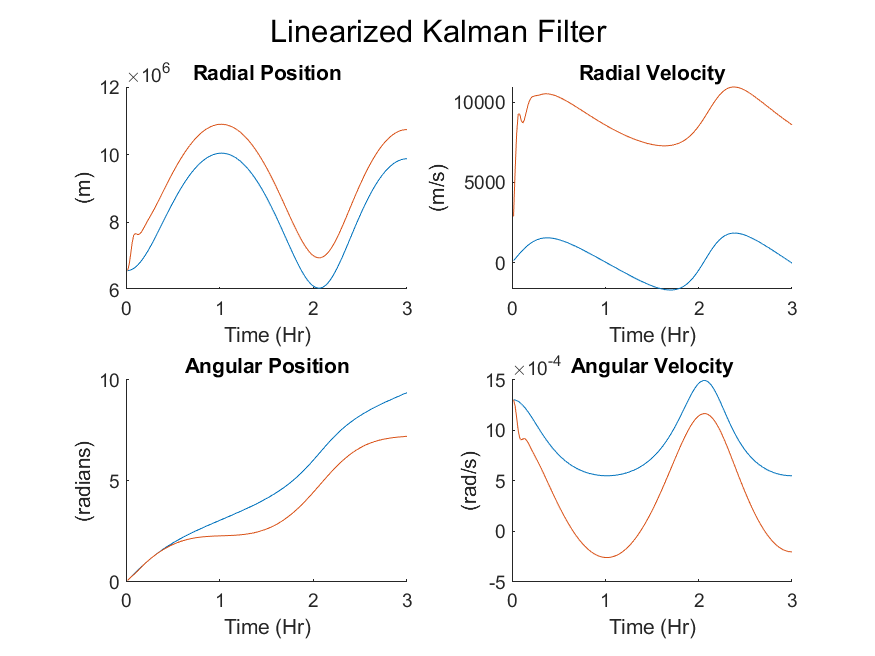
\includegraphics[width=1.2\textwidth]{MATLAB/fig/pblm5_results_hybrid_lin}}
			\caption{Simulation Results for the Linear Hybrid \KF \ for problem 5}
			\label{fig:pblm5resultslin}
		\end{figure}
	
	\newpage
		The estimation error for the Linear Hybrid \KF \ can be seen in \figurename \ \ref{fig:pblm5esterrorlin}.\\
		\begin{figure}[h]
			\centering
			\makebox[\textwidth][c]{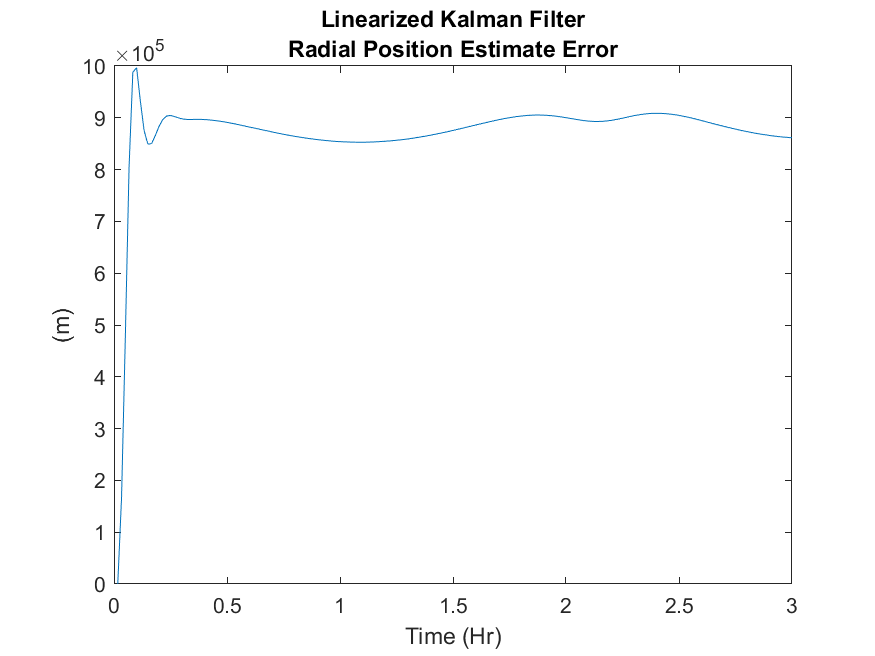
\includegraphics[width=1.2\textwidth]{MATLAB/fig/pblm5_est_error_hybrid_lin}}
			\caption{Estimation Error for the Linear Hybrid \KF \ for problem 5}
			\label{fig:pblm5esterrorlin}
		\end{figure}
	
		The performance of the linear Kalman Filter is reduced by the lack of linearity in the actual system dynamics. This may be improved with faster measurments and Kalman Filter updates; however this is not guaranteed. Using an Extended \KF \ would be the better solution.
	
	\newpage
		\subsubsection{Hybrid Extended \KF}
		The Hybrid Extended \KF \ was simulated using \subsectionname \ \ref{sec:HybridEKF}. The system response can be seen in \figurename \ \ref{fig:pblm5resultsEKF}.
		\begin{figure}[h]
			\centering
			\makebox[\textwidth][c]{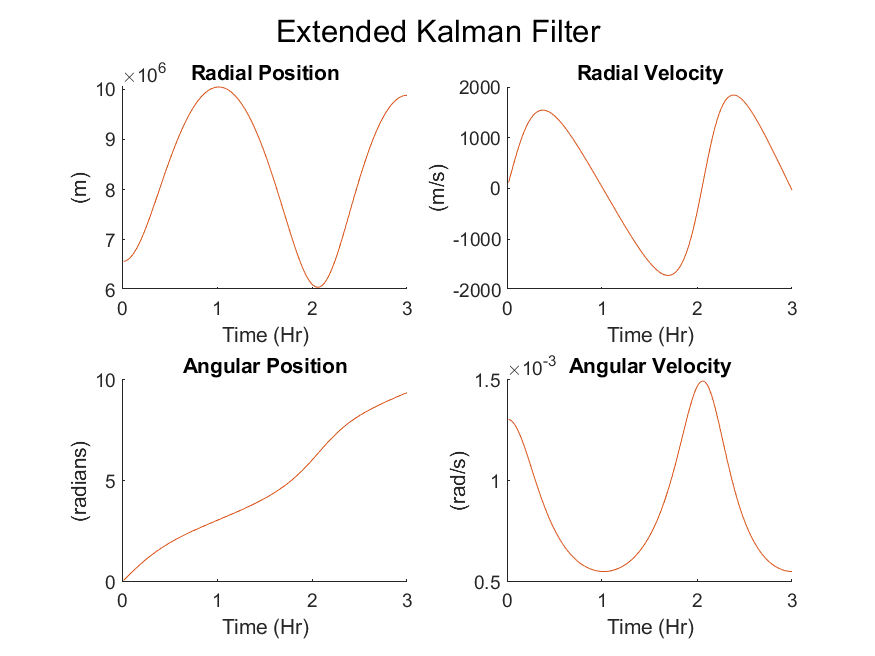
\includegraphics[width=1.2\textwidth]{MATLAB/fig/pblm5_results_hybrid_EKF}}
			\caption{Simulation Results for the Hybrid Extended \KF \ for problem 5}
			\label{fig:pblm5resultsEKF}
		\end{figure}
	\newpage
		The estimation error for the Hybrid Extended \KF \ can be seen in \figurename \ \ref{fig:pblm5esterrorEKF}.\\
		\begin{figure}[h]
			\centering
			\makebox[\textwidth][c]{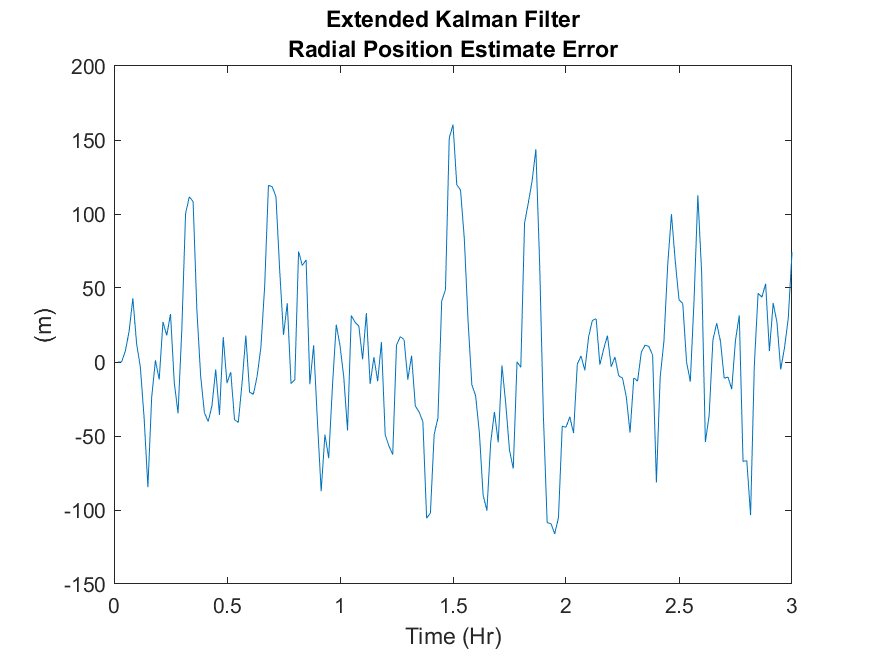
\includegraphics[width=1.2\textwidth]{MATLAB/fig/pblm5_est_error_hybrid_EKF}}
			\caption{Estimation Error for the Hybrid Extended \KF \ for problem 5}
			\label{fig:pblm5esterrorEKF}
		\end{figure}
		
		It is clear that the Extended \KF \ performs much better then the Linear one. Although the error is more sporadic, the magnitude is order smaller then the linear one. This is likely due to the ability for the Extended \KF \ to account for the non linear dynamics during the time-update stage.
		
\newpage
\appendix
\section{MATLAB Code} \label{apx:MATLAB_Code}
	
	% MECH6325_FinalProject.m
	\lstinputlisting[caption={MECH6325\_FinalProject.m},label={script:FinalProject}]{MATLAB/MECH6325_FinalProject.m}
	
	\newpage
	\subsection{Problem 1}
	% pblm1.m
	\lstinputlisting[caption={pblm1.m},label={script:pblm1}]{MATLAB/pblm1.m}
	\newpage
	% KalmanFilter_DT.m
	\lstinputlisting[caption={KalmanFilter\_DT.m},label={script:KF_DT}]{MATLAB/KalmanFilter_DT.m}
	
	\newpage
	\subsection{Problem 2}
	% pblm2.m
	\lstinputlisting[caption={pblm2.m},label={script:pblm2}]{MATLAB/pblm2.m}
	\newpage
	% DiscretizeSystem.m
	\lstinputlisting[caption={DiscretizeSystem.m.m},label={script:DiscretizeSystem}]{MATLAB/DiscretizeSystem.m}
	\newpage
	% KalmanFilter_Sequential.m
	\lstinputlisting[caption={KalmanFilter\_Sequential.m},label={script:KF_Sequential}]{MATLAB/KalmanFilter_Sequential.m}
	
	\newpage
	\subsection{Problem 3}
	% pblm3.m
	\lstinputlisting[caption={pblm3.m},label={script:pblm3}]{MATLAB/pblm3.m}
	
	\newpage
	\subsection{Problem 4}
	% pblm4.m
	\lstinputlisting[caption={pblm4.m},label={script:pblm4}]{MATLAB/pblm4.m}
	\newpage
	% KalmanFilter_DT_SDS.m
	\lstinputlisting[caption={KalmanFilter\_DT\_SDS.m},label={script:KF_DT_SDS}]{MATLAB/KalmanFilter_DT_SDS.m}	
	
	\newpage
	\subsection{Problem 5}
	% pblm5.m
	\lstinputlisting[caption={pblm5.m},label={script:pblm5}]{MATLAB/pblm5.m}
	\newpage
	% pblm5_nonlin.m
	\lstinputlisting[caption={pblm5\_nonlin.m},label={script:pblm5_nonlin}]{MATLAB/pblm5_nonlin.m}
	\newpage
	% KalmanFilter_Hybrid_nonlinsys.m
	\lstinputlisting[caption={KalmanFilter\_Hybrid\_nonlinsys.m},label={script:KF_Hybrid_nonlinsys}]{MATLAB/KalmanFilter_Hybrid_nonlinsys.m}
	\newpage
	% KalmanFilter_Extended_Hybrid.m
	\lstinputlisting[caption={KalmanFilter\_Extended\_Hybrid.m},label={script:KF_Extended_Hybrid}]{MATLAB/KalmanFilter_Extended_Hybrid.m}

\section{MATLAB Output}
	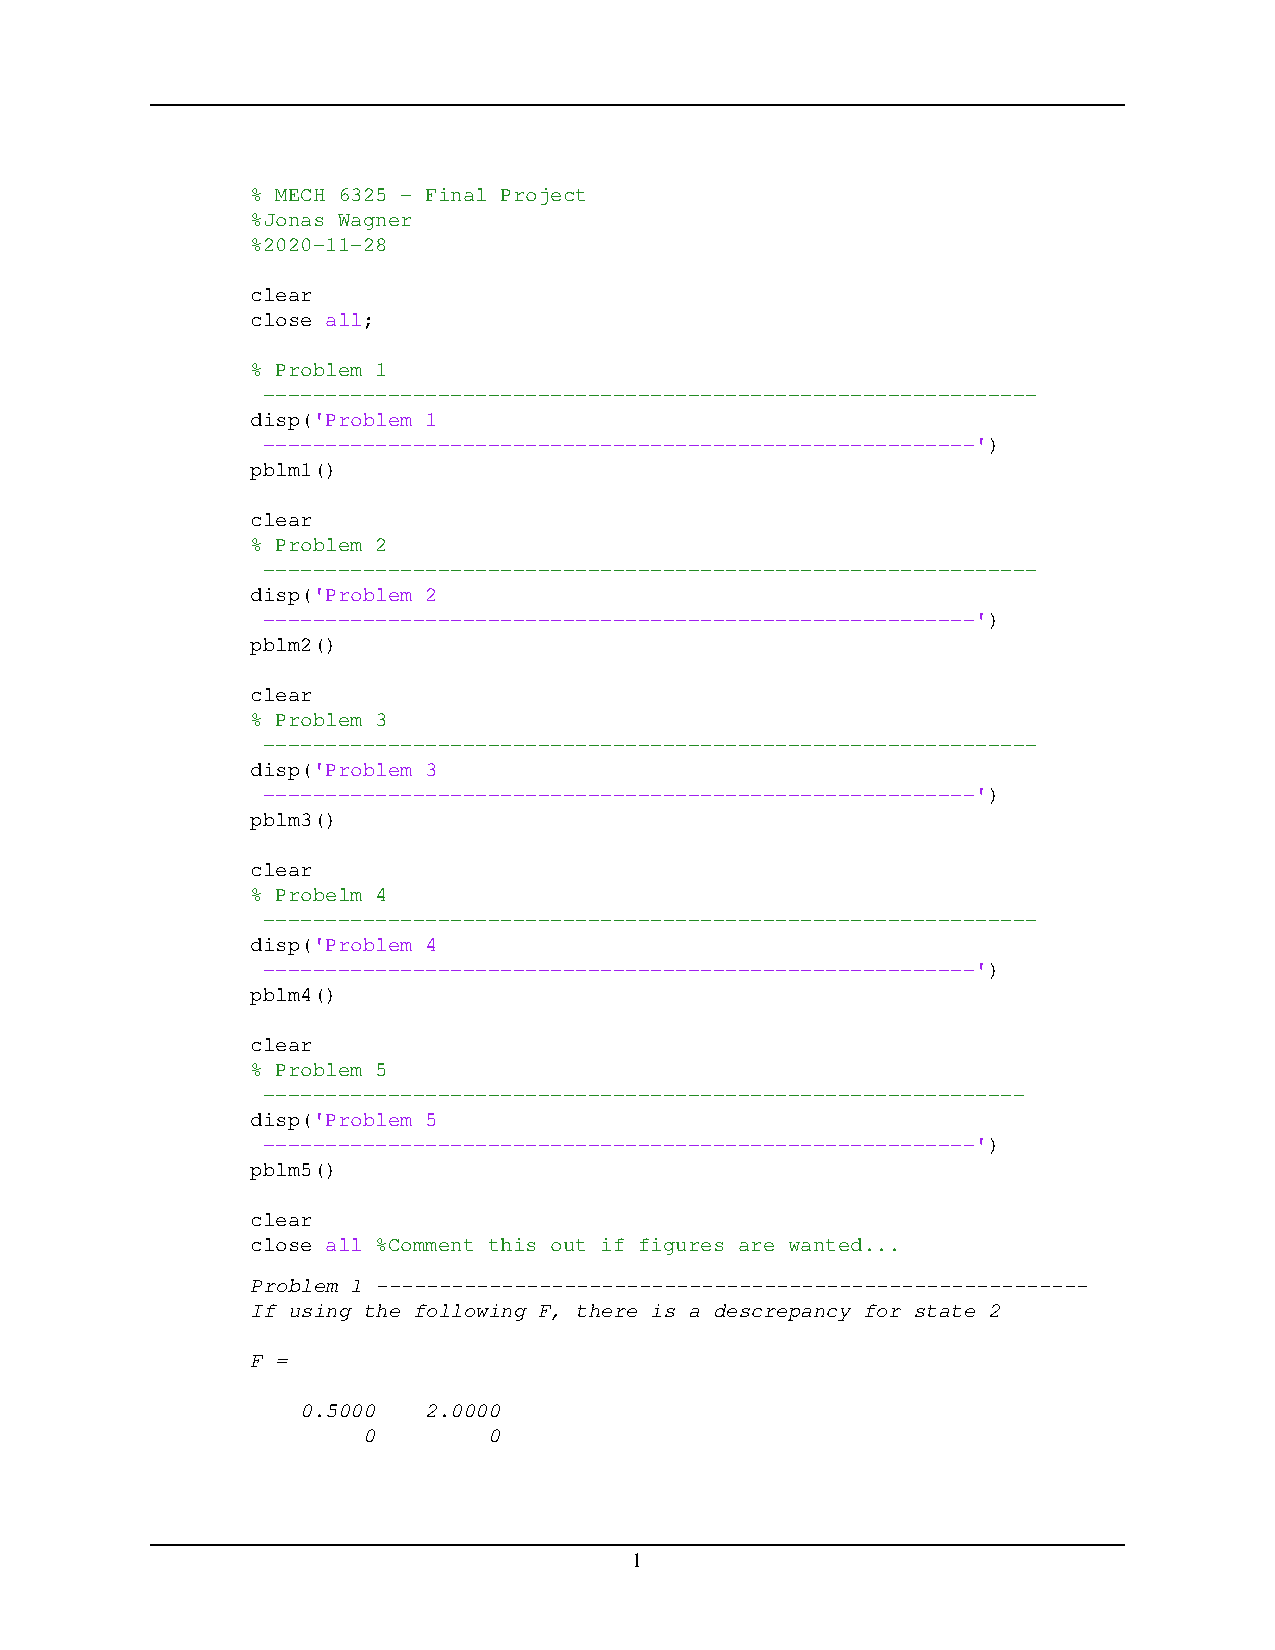
\includepdf[pages=-]{MATLAB/html/MECH6325_FinalProject.pdf}
	
\section{Hand Calculations}
	\includepdf[pages=-]{MECH6325-FinalProject_handCalc.pdf}
\end{document}
